\documentclass[10pt,a4paper]{article}
\usepackage[margin=25.4mm]{geometry}
\usepackage{graphicx,float,booktabs}
\usepackage{tikz}
\title{Structure and Meta-Information Cleanup}
\author{Sh Lab}
\date{}
\begin{document}
\maketitle

START READING HERE

\section{Introduction}
The manuscript that follows was assembled by an editor who left several pieces
of scaffolding in the file. The reader of the final paper should never see them.

WARNING: the numbers in Table 1 were regenerated after the deadline and have not
been re-checked by the second author.

\begin{table}[tbp]\centering
\caption{A placeholder table kept for review.}
\begin{tabular}{ll}\toprule Key & Value \\\midrule alpha & 1 \\ beta & 2 \\\bottomrule
\end{tabular}
\end{table}

CAUTION: this figure must be replaced before submission, the current version is
only a draft rendering.

\begin{figure}[tbp]\centering
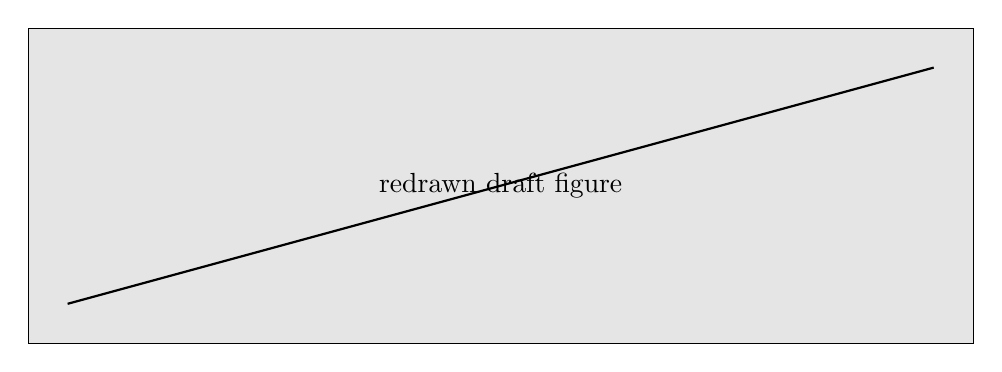
\begin{tikzpicture}
\draw[fill=gray!20] (0,0) rectangle (12,4);
\draw[thick] (0.5,0.5) -- (11.5,3.5);
\node at (6,2) {redrawn draft figure};
\end{tikzpicture}
\caption{A draft figure that is wider than the text block.}
\end{figure}
Layout optimization for academic manuscripts is a constrained problem: the visual result of a document is a global property of the whole file, while most editing actions are local. A change that removes one bad line can push a float to the next page and create a much larger gap, so an optimizer must always recompile and re-evaluate the entire document before accepting an edit.

The scoring model used here separates logic from aesthetics. Logic asks whether the file compiles, whether the rendered PDF keeps the body text byte-identical, and whether the requested hard constraints such as font size, margins and page limits are satisfied. Aesthetics collects measurable layout defects such as overfull lines, underfull lines, badly placed floats and inconsistent vertical spacing.

Intervention cost makes the optimizer conservative. Every edit that is applied to the source increases the intervention score, so a repair is only kept when the total objective improves after a full recompilation. This is what prevents the system from grooming its own score with edits that no human would ever make.

\newpage

\section{Method}
Page limits deserve special care. Compressing a document by shrinking its margins changes the relationship between floats and the text that refers to them, and the resulting layout often looks wrong even though every number in the report is legal. For that reason the default policy refuses to touch the global text block and reports an honest failure instead.

The pipeline is deterministic. Given the same source file, the same requirement specification and the same toolchain, it produces the same trace of candidate actions, the same accept and rollback decisions, and the same final document. Determinism matters for reproducibility, for regression testing and for the audit trail that is written next to every run.

Perception is layered. The source layer parses the LaTeX file and looks for patterns that are known to be unstable, such as manual page breaks, manual vertical spacing, bare dollar math and float specifications that pin a float to its declaration point. The log layer reads the compiler log and counts overfull boxes, underfull boxes and badness warnings.

The rendered layer measures the PDF itself. Page images give coverage statistics, the vertical position of ink, and the size of the largest empty band on each page. Those numbers are coarse on purpose: they are used as evidence that something looks wrong, not as a model of human taste.

Float placement is the hardest part of the problem. A figure that is referenced in one paragraph may be typeset several pages later, and the quality of the page depends on whether the top, bottom and text fraction constraints of the float mechanism are balanced. Sanitising the float specification to the top, bottom and page forms is a cheap first step.

Perception is layered. The source layer parses the LaTeX file and looks for patterns that are known to be unstable, such as manual page breaks, manual vertical spacing, bare dollar math and float specifications that pin a float to its declaration point. The log layer reads the compiler log and counts overfull boxes, underfull boxes and badness warnings.

The rendered layer measures the PDF itself. Page images give coverage statistics, the vertical position of ink, and the size of the largest empty band on each page. Those numbers are coarse on purpose: they are used as evidence that something looks wrong, not as a model of human taste.


\section{Results}
Intervention cost makes the optimizer conservative. Every edit that is applied to the source increases the intervention score, so a repair is only kept when the total objective improves after a full recompilation. This is what prevents the system from grooming its own score with edits that no human would ever make.

Page limits deserve special care. Compressing a document by shrinking its margins changes the relationship between floats and the text that refers to them, and the resulting layout often looks wrong even though every number in the report is legal. For that reason the default policy refuses to touch the global text block and reports an honest failure instead.

The pipeline is deterministic. Given the same source file, the same requirement specification and the same toolchain, it produces the same trace of candidate actions, the same accept and rollback decisions, and the same final document. Determinism matters for reproducibility, for regression testing and for the audit trail that is written next to every run.

Perception is layered. The source layer parses the LaTeX file and looks for patterns that are known to be unstable, such as manual page breaks, manual vertical spacing, bare dollar math and float specifications that pin a float to its declaration point. The log layer reads the compiler log and counts overfull boxes, underfull boxes and badness warnings.

The rendered layer measures the PDF itself. Page images give coverage statistics, the vertical position of ink, and the size of the largest empty band on each page. Those numbers are coarse on purpose: they are used as evidence that something looks wrong, not as a model of human taste.


\section{Conclusion}
Once the scaffolding is gone and the figure is renormalised, the document is a
plain article again.
\end{document}
